\newpage
\subsection{QuizziPedia::Front-End::Services}
\begin{figure}[ht]
	\centering
	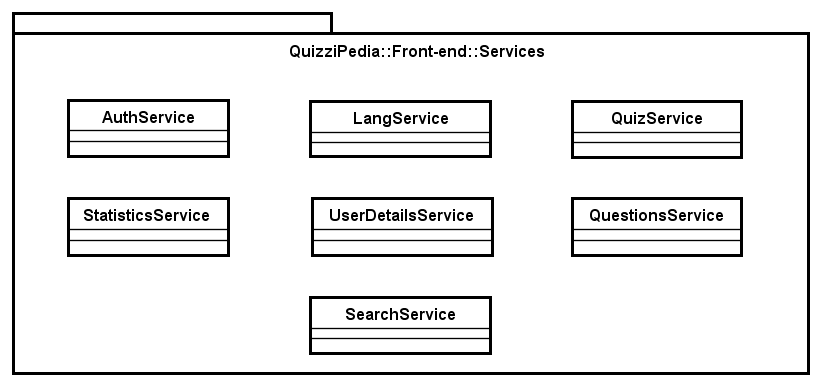
\includegraphics[scale=0.55]{UML/Package/QuizziPedia_Front-End_Services.png}
	\caption{QuizziPedia::Front-End::Services}
\end{figure} \FloatBarrier

\begin{itemize}
	\item \textbf{Descrizione}: package che contiene le classi individuate che permettono la comunicazione del lato front-end con il lato back-end;
	\item \textbf{Padre:} \texttt{Front-End};
	\item \textbf{Interazione con altri componenti:}
	\begin{itemize}
		\item \texttt{Models}: package che contiene le classi \textit{model\ped{G}} dell'applicazione;
		\item \texttt{Controllers}: package che contiene le classi \textit{controller\ped{G}} dell'applicazione.
	\end{itemize}
	\item \textbf{Classi contenute}:
	\begin{itemize}
		\item \texttt{AuthServices}: questa classe permette di gestire la registrazione e l'autenticazione di un utente;
		\item \texttt{LangService}: questa classe permette di gestire la lingua nella quale si è scelto di utilizzare l'applicazione;
		\item \texttt{QuestionsService}: questa classe permette di ottenere domande esistenti e salvare nuove domande;
		\item \texttt{QuizService}: questa classe permette di ottenere i dati di un quiz tramite delle parole chiave inserite dall'utente nella barra di ricerca. Permette inoltre di iscriversi ad un questionario e di scaricare l'intera lista di domande di un questionario a partire dal suo id univoco;
		\item \texttt{SearchService}: questa classe permette di gestire il recupero dei dati dal back-end a seguito di una ricerca effettuata da un utente;
		\item \texttt{StatisticsService}: questa classe permette di ottenere le statistiche dell'utente;
		\item \texttt{UserDetailsService}: questa classe permette di ottenere i dati personali degli utenti.
	\end{itemize} 
\end{itemize}